\chapter{Implementation}

\section{Design and Conception}

We are now focusing on the design and concept of the application. On an abstract level, the application should be a REST API with a database to store users, items and user ratings. This data should be available on the API along with recommendations and similarities.

\begin{figure}[h]
\centering
\includegraphics[width=\textwidth]{images/BPMN_design}
\caption{\label{fig:design}description}
\end{figure}

\subsection{Routing}

Let's take a closer look at all the web routes and how they work and what they provide.

For user data, there should be the following web routes:

\begin{longtable}{|p{2.5cm}|p{2.5cm}|p{3.2cm}|p{5cm}|}
    \hline
	  Name & Http Method & Route & Description \\
    \hline
    \hline
    User Info & GET & /user/<userid> & Returns the username and optional information of the user\\
    \hline
    User ratings & GET & /user/ratings & Should provide all ratings of all users\\
    \hline
    Create User & PUT & /user & Should create a user, and takes a data object for name and in formations\\
    \hline
    Add rating & POST & /user/rating & Should create ratings defined in a data object\\
    \hline
    All users & GET & /users & Returns all users (id, name, information)\\
    \hline
\end{longtable}

For the items we define the following web routes:

\begin{longtable}{|p{2.5cm}|p{2.5cm}|p{3.2cm}|p{5cm}|}
    \hline
	  Name & Http Method & Route & Description \\
    \hline
    \hline
    User Info & GET & /item/<itemId> & Returns item name and description\\
    \hline
    Create item & PUT & /item & Creates a item and takes the name and description form the provided data\\
    \hline
    Modify item & POST & /item & Updates the description and name of an item\\
    \hline
    All items & GET & /items & Returns all items (id, name, description)\\
    \hline
\end{longtable}

We also define the routes for the recommender system:

\begin{longtable}{|p{2.5cm}|p{2.5cm}|p{3.2cm}|p{5cm}|}
    \hline
	  Name & Http Method & Route & Description \\
    \hline
    \hline
    User Similarities & GET & /userBased/\allowbreak similarities/\allowbreak<userid> & Returns all user similarities to the specified user\\
    \hline
    Userbased Recommendations & GET & /userBased/\allowbreak recommendations/\allowbreak<userid> & Returns all unrated items of the specified user with an estimated rating\\
    \hline
    Items Similarities & GET & /userBased/\allowbreak similarities/\allowbreak<itemId> & Returns all item similarities to the specified item\\
    \hline
    Itembased Recommendations & GET & /userBased/\allowbreak recommendations/\allowbreak <itemId> & Returns all unrated items of the specified user with an estimated rating\\
    \hline
\end{longtable}

\subsection{Recommender}

We will now look at the design of the recommender system. We divide the recommender system into components: 

\begin{itemize}
    \item A controller that takes all the data and feeds it to all the necessary components
    \item The similarity measure, which allows the recommender system to compare two users or items
    \item election algorithms to select only the most relevant items and users to make a recommendation
\end{itemize}

The interactions and relationships between the components are shown in \ref{fig:recommender_design}.

\begin{figure}[h]
\centering
\includegraphics[width=\textwidth]{images/BPM_recommender_design}
\caption{\label{fig:recommender_design}description}
\end{figure}


\section{Technologies}

\subsection{Kotlin Framework Ktor}

Ktor is a web framework for building web services, clients or applications connected over the web. Ktor uses coroutines to achieve an asynchronous context to provide an efficient framework for developers.

In this paper we will mainly use the Ktor server dependencies, and only use the Ktor client if the application needs to make requests to other services itself.

\subsection{Kotlin Library Ktorm}

Ktorm is a database ORM for SQL databases written in Kotlin. It provides a strongly typed SQL DSL for constructing SQL queries (https://www.ktorm.org/). A DSL or type-safe builder (https://kotlinlang.org/docs/type-safe-builders.html) can help to provide a builder that is statically typed and type-safe. This forces a developer to write correct SQL statements.

Ktorm also handles the connection to the database and keeps the tables as Kotlin objects for easy interaction with the database.

\subsection{Ktor Plugins}

Additional dependencies we use are available as Ktor plugins, this way the Ktor framework handles the initialisation of these dependencies and provides them when needed.

\subsubsection{Koin}

Koin is a dependency injection framework that is available for the Kotlin programming language (https://insert-koin.io/). In this Application we use Koin to manage Objects like a Database object that is shared between asynchronous Route Objects and make it accessible.

We start Koin at the start of the application within Ktor:

\begin{minted}{kotlin}
fun Application.configureKoin(vararg appModules: Module) {
    install(Koin) {
        slf4jLogger()
        modules(appModules.toList())
    }
}
\end{minted}

We define the app module before we start the Ktor application:

\begin{minted}{kotlin}
    val config = ConfigLoader().loadConfig().getOrElse { it ->
        log.error(it.message)
        this.dispose()
        return
    }
    val logger = LoggerFactory.getLogger("api")

    val appModules = org.koin.dsl.module {
        single { config }
        single(qualifier("main")) { config.databases.main }
        single { logger }
        single { BpmDatabase() }
        single { JwtConfig(config.token) }
    }
\end{minted}


\subsubsection{CORS}

The application also defines CORS or Cross-Origin Resource Sharing. This is where the main application simply references the API in the browser so that the client makes the request to the API itself. The author strongly recommends making the API request from the server backend and not letting the client handle it, as the API was not designed with this in mind.

When deploying the application, allowed hosts can be defined in the config.yaml.

\subsubsection{Authentication}

For the authentication to access the different routes on the API Json Web Tokens or JWT is used. To configure this feature we also just install the authentication plugin with JWT.

\begin{minted}{kotlin}
fun Application.configureSecurity(jwtConfig: JwtConfig) {
    authentication {
        jwt {
            jwtConfig.configureKtorFeature(this)
        }
    }
}
\end{minted}

In this case more configuration is needed as we can save some data into the JWT to access this data within a request. THe JWT configuration can be found int appendix \ref{code:JWT_conf}.

\subsubsection{Serialization}

The application uses JSON as Content Negotiation as defined in the functional requirements. The kotlin serialization plugin in combination with Ktorm enables the Application to send Kotlin Objects while the serialization plugin transform the objects to JSON and also transforms JSON within a http body to Kotlin object. 

\begin{minted}{kotlin}
fun Application.configureSerialization() {
    install(ContentNegotiation) {
        json()
    }
}
\end{minted}

\section{Architecture}

In this section we try to implement what we have defined in the conception phase. We also define other necessary components that are relevant, such as dependencies or the server framework. 

\subsection{Application Startup}

To start the application, the application configuration has to be loaded. This can happen three different ways as shown in \ref{fig:startup}.

\begin{figure}[h]
\centering
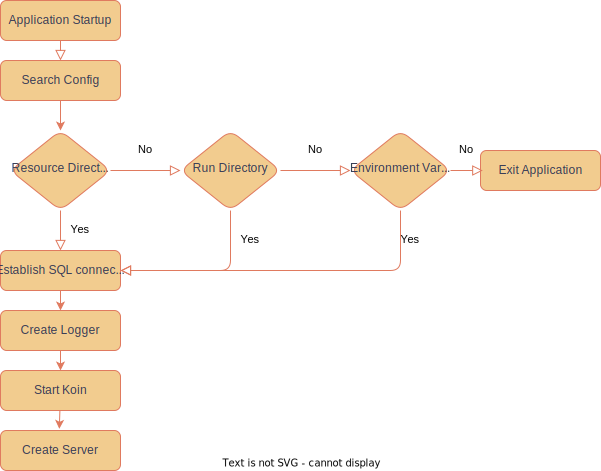
\includegraphics[width=\textwidth]{images/StartupBachelor.drawio.png}
\caption{\label{fig:startup}description}
\end{figure}

The configuration loading process is shown in \ref{code:App_conf_loading}.

\subsection{Routing}

see image: \ref{fig:routing}

\begin{figure}[ht]
\centering
\includegraphics[width=\textwidth]{images/RoutingUML.png}
\caption{\label{fig:routing}Routing UML class diagram}
\end{figure}


\subsection{Database Access Objects}

We change the dataflow described in the design section and introduce a database access object that contains all the queries we need as seen in \ref{fig:dao_vis}.

\begin{figure}[ht]
\centering
\includegraphics[width=\textwidth]{images/dao_visualizer.png}
\caption{\label{fig:dao_vis}Database Access Object}
\end{figure}

Within the DAO, we now define queries using the Ktrom ORM DSL, for example to get all users:

\begin{minted}{kotlin}
fun getAllUsers(): EntitySequence<UserDbEntity, UserDbTable> {
    return database.sequenceOf(UserDbTable)
}
\end{minted}

\section{Recommendation Algorithms}

\subsection{Similarity Measures}

All similarity measures implement an interface to facilitate the use of the algorithms.

\begin{minted}{kotlin}
interface SimilarityMeasure {
    /**
     * compares 2 data maps and returns a similarity measure,
     * note: comparing the result of this function only works 
     * with the same Similarity Measure!
     *
     * @param dataA the first data set
     * (key: the item, value: the rating of the item)
     * @param dataB the second data set
     * (key: the item, value: the rating of the item)
     * @param allItems all the items referenced in data1 & 2
     */
    fun compare(
        dataA: Map<String, Int>,
        dataB: Map<String, Int>,
        allItems: List<String>
    ): Number
}
\end{minted}

\subsubsection{Euclid}

The Euclidean algorithm can calculate similarity based on distance. In other words, if the distance between two users is small, they are more similar. The dimension n is the number of items.

\begin{equation}
S_{e} = \frac{1}{1+\sqrt{\sum_{i=1}^{n}{(dataA_i - dataB_i)^2}}}
\label{euklid}
\end{equation}

DataA and DataB refer to the ratings of two different users or items.
The implementation in Kotlin is as follows:

\begin{minted}{kotlin}
class Euclid : SimilarityMeasure {
    override fun compare(
        dataA: Map<String, Int>,
        dataB: Map<String, Int>,
        allItems: List<String>,
    ): Number {
        val sum = allItems.sumOf {
            ((dataA[it] ?: 0) - (dataB[it] ?: 0))
                .toDouble().pow(2)
        }

        return 1 / (1 + sqrt(sum))
    }
}
\end{minted}

The difference of the ratings of DataA and DataB is an integer, but is converted to a double because the pow() function in the Kotlin standard library is only defined for floats and doubles.

\subsubsection{Cosine}

The basic calculation is separated into the companion object of the class as the calculation is also used by the Pearson distance measure. 

\begin{minted}{kotlin}
//TODO formatting
class Cosine : SimilarityMeasure {
    companion object {
        fun basicCalc(
            dataA: Map<String, Number>,
            dataB: Map<String, Number>,
            allItems: List<String>,
        ): Number {
            var sumATimesB = 0.0
            var sumASquared = 0.0
            var sumBSquared = 0.0

            allItems.forEach {
                sumATimesB += (dataA[it] ?: 0).toDouble() * (dataB[it] ?: 0).toDouble()
                sumASquared += (dataA[it] ?: 0).toDouble().pow(2)
                sumBSquared += (dataB[it] ?: 0).toDouble().pow(2)
            }

            return (sumATimesB / (sqrt(sumASquared * sumBSquared)))
        }
    }

    override fun compare(
        dataA: Map<String, Int>,
        dataB: Map<String, Int>,
        allItems: List<String>,
    ): Number {
        return basicCalc(dataA, dataB, allItems)
    }
}
\end{minted}

\subsubsection{Pearson}

\subsection{Knn}

\subsection{Mean/Average}
